\documentclass[a4paper,12pt]{article}
 \usepackage[utf8]{inputenc}
 \usepackage[left=2cm,top=1cm,right=2cm,bottom=1.5cm,nohead]{geometry}
%\usepackage{wrapfig} % Обтекание рисунков текстом
%\usepackage{floatflt}% Обтекание таблиц текстом
 \usepackage{amsmath} % Математические окружения AMS
 \usepackage{amsfonts} % Шрифты AMS
 \usepackage{amssymb} % Символы AMS
 \usepackage{listings}% to add computer code
 \usepackage{color}
 \definecolor{mygreen}{RGB}{28,172,0} % color values Red, Green, Blue
\definecolor{mylilas}{RGB}{170,55,241}
    \usepackage{graphicx} % Вставить pdf- или png-файлы
  \usepackage{euscript} % Красивый шрифт
%\usepackage{extsizes} % Возможность сделать 14-й шрифт
 \linespread{1.5} % Интерлиньяж
% \usepackage[usenames,dvipsnames,svgnames,table,rgb]{xcolor}% чтоб были гиперссылки и чтоб были цвета

\usepackage{hyperref} % Гиперссылки

%\hypersetup{
% colorlinks = true,
 %linkcolor = MidnightBlue, % ссылки на всякие разделы (их цвет)
 %urlcolor = [rgb]{0,0,1}, % чтоб задавать цыета пиксела - red green blue. не рекомендуется, если потом печатать.
 %citecolor = black
%}
%\usepackage{pdflscape}
%\oddsidemargin=10mm
%\topmargin=-15mm
\usepackage{multicol}
%\hoffset=5mm % см при печати
%\voffset=4.2mm
%\textheight = 720pt
%\textwidth=442pt

\begin{document}
\maketitle \hrulefill
\lstset{language=Matlab,%
    %basicstyle=\color{red},
    breaklines=true,%
    morekeywords={matlab2tikz},
    keywordstyle=\color{blue},%
    morekeywords=[2]{1}, keywordstyle=[2]{\color{black}},
    identifierstyle=\color{black},%
    stringstyle=\color{mylilas},
    commentstyle=\color{mygreen},%
    showstringspaces=false,%without this there will be a symbol in the places where there is a space
    numbers=left,%
    numberstyle={\tiny \color{black}},% size of the numbers
    numbersep=9pt, % this defines how far the numbers are from the text
    emph=[1]{for,end,break},emphstyle=[1]\color{red}, %some words to emphasise
    %emph=[2]{word1,word2}, emphstyle=[2]{style},
}

\begin{center}

\textbf {\Large{Empirircal Methods HA 2}}\\
Konstantin Guryev\\
Pennsylvania State University\\
2018
\end{center}

\textbf{Problem \textnumero \,1 }

\vspace{\baselineskip}
\begin{pmatrix}
  D_{A} \\
  D_{B}\\
  D_{0}
\end{pmatrix}
 =
\begin{pmatrix}
  0.4223 \\
  0.4223\\
  0.1554
\end{pmatrix};
\vspace{\baselineskip}

\textbf{Problem \textnumero \,2 }

\vspace{\baselineskip}
The starting values are: $p_{A}=p_{B}=2$; $v_{A}=v_{B}=2$. Nash pricing equilibrium: $p_{A}=p_{B}= 1.598942$. Number of iterations needed for convergence is equal to $5$ for the chosen starting values. Elapsed time (for 5 compilations) varied from 0.009430 to 0.064949 seconds. I tried other starting values for $p$, but the numerical solution for NE vector of prices is the same. Tolerance level is set to be equal to $1e-10$.
\vspace{\baselineskip}

\textbf{Problem \textnumero \,3 }

\vspace{\baselineskip}
The Gauss-Seidel method converges in 40 iterations, but the elapsed time (for 5 compilations) varied from 0.010673 to 0.019461. The equilibrium price values are the same as for Broyden's method. We can conclude that The G-S method is on average faster than Broyden's method. The latter approximates the whole Jacobian whereas G-S does not - that is the reason why G-S is faster.
\vspace{\baselineskip}

\textbf{Problem \textnumero \,4 }

\vspace{\baselineskip}
The proposed updating rule method converges in $18$ iterations an the elapsed time (for 5 compilations) varied from 0,007514 to 0,008043. So we can conclude that this method is faster than the other two methods. The equilibrium price values are the same as in the previous calculations.
\vspace{\baselineskip}

\textbf{Problem \textnumero \,5 }

\vspace{\baselineskip}
I solved the task using Broyden's method. The results are on the graph:

\begin{figure}[h]
\centering
%\begin{center}
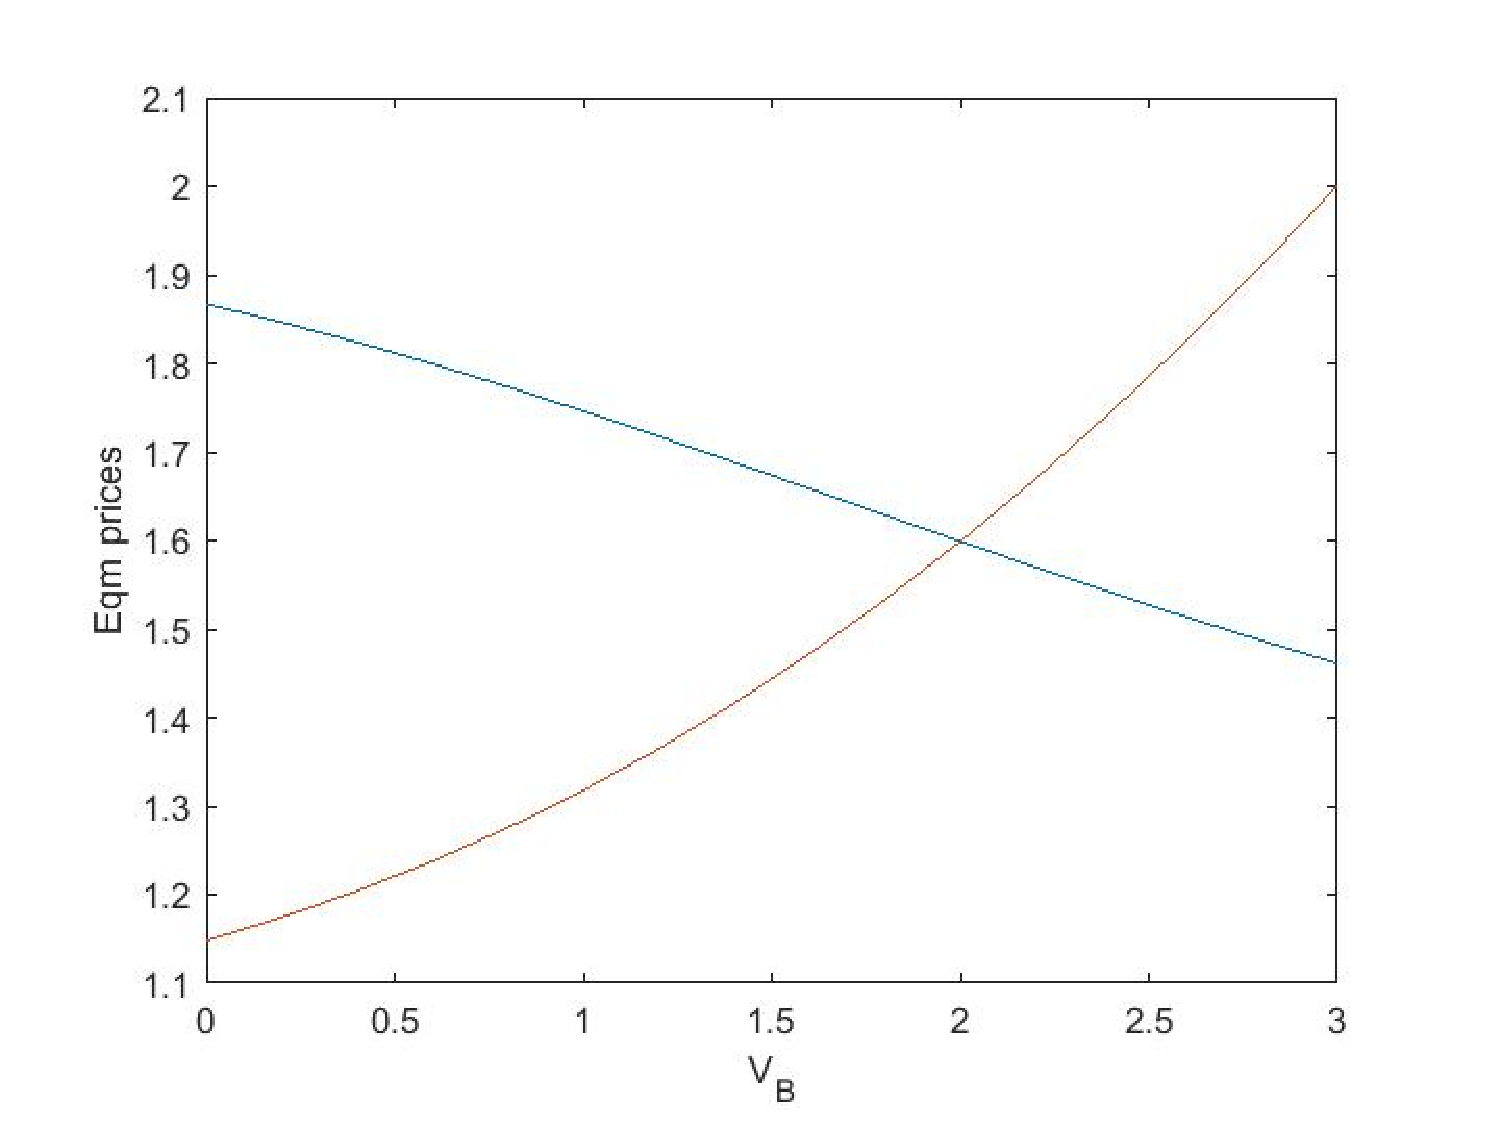
\includegraphics[width=16cm,height=8cm,keepaspectratio]{Equilibrium.eps}
%\caption{Движущийся жесткий штамп}
%\caption{pic1}
%\end{center}
\end{figure}
\vspace{\baselineskip}

\newpage
\section*{Matlab Code} \lstinputlisting{FOC.m}
\newpage
\section*{Matlab Code} \lstinputlisting{br.m}
\newpage
\section*{Matlab Code} \lstinputlisting{HA_2_Guryev.m}


\end{document}